\section{Helper Definitions}
    
    Before we go into the consistency rules. we define certain preliminary definitions that create a separation based on a program, the axiomatic events and the various ordering relations defined above. This will help us understand where the consistency rules actually apply.    
    
    %What is a program 
    \begin{definition}{Program} 
        A \emph{program} is the source code without abstraction to a set of events and ordering relations. In our context, it is the original Javascript program. 
        
        %Note that here we need to supply a Javascript program using shared array buffers and atomic objects. A thing to do after we give examples for the ones below
    \end{definition}
    
%-----------------------------------------------------------------------------------------------------------------------------------------    
    %What is one run of a program to us?
    \begin{definition}{Candidate}
        A a collection of abstracted set of shared memory events of a program involved in one possible execution, with the $\stck{_\textit{ao}}$ relations. 
        We can think of this as each thread having a set of shared memory events to run in a given intra-thread ordering. 
        Figure~\ref{model:candidate} is an example of a Candidate.
        \begin{figure}[H]
            \centering
            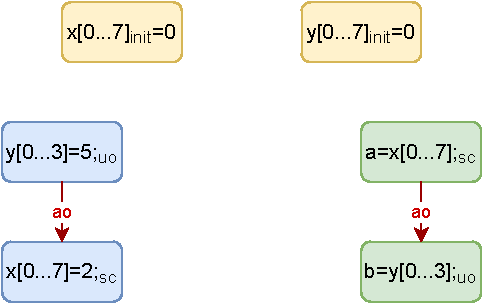
\includegraphics[scale=0.7]{3.ECMAScriptMemoryModel/candidate.pdf}
            \caption{An example of a Candidate.}
            \label{model:candidate}
        \end{figure}
        
    \end{definition}

%-----------------------------------------------------------------------------------------------------------------------------------------  
    \begin{definition}{Candidate Execution}
        A Candidate with the addition of $\stck{_\textit{sw}}$, $\stck{_\textit{hb}}$ and $\stck{_\textit{mo}}$ relations. 
        This can be viewed as the witness/justification of an actual execution of a Program. 
        Note that there can be many Candidate Executions for a given Candidate. 
        Figure~\ref{model:candexec} shows an example of a Candidate Execution.  
        \begin{figure}[H]
            \centering
            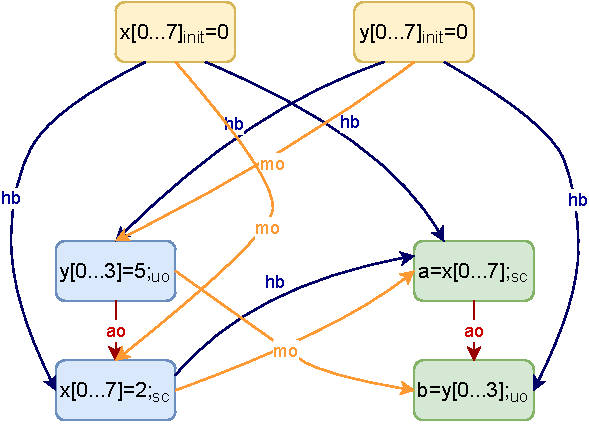
\includegraphics[scale=0.7]{3.ECMAScriptMemoryModel/CandidateExecution.pdf}
            \caption{An example of a Candidate Execution based on Candidate above.}
            \label{model:candexec}
        \end{figure}
        
    \end{definition}

 %-----------------------------------------------------------------------------------------------------------------------------------------   
    %What values are read when the program is run
    \begin{definition}{Observable Behavior}
        The set of pairwise $\stck{_\textit{rf}}$/$\stck{_\textit{rbf}}$ relations that result in one execution of the program. 
        Think of this as our outcome of a program execution.
        Figure~\ref{model:observable} shows an example of an observable behavior.
        \begin{figure}[H]
            \centering
            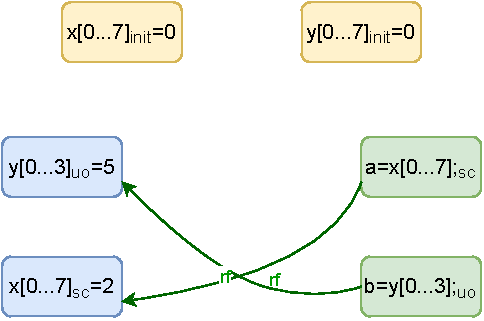
\includegraphics[scale=0.7]{3.ECMAScriptMemoryModel/Observables.pdf}
            \caption{An example of Observable Behavior.}
            \label{model:observable}
        \end{figure}
        
    \end{definition}

%-----------------------------------------------------------------------------------------------------------------------------------------
    